
\begin{figure}[H]
	\centering
	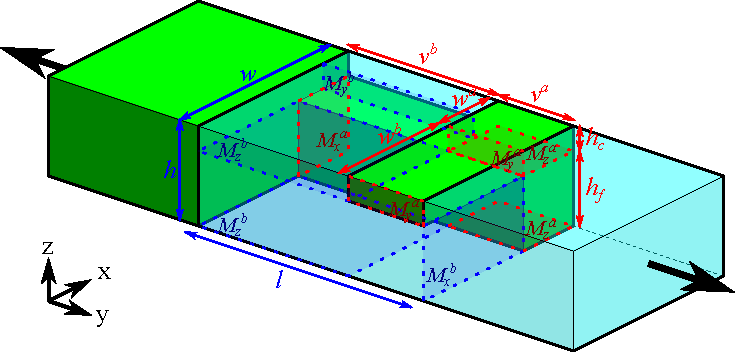
\includegraphics[width=\columnwidth]{sources/method/straight_model_v3.pdf}
	\caption{
		One straight unit cell connecting material $a$ (left) to material $b$ (right).
		Failure can happen along the fingers ($M_x$), along the cross beams ($M_y$) or at the interface between the two ($M_z$) for either material.}
	\label{fig:failure_modes}
\end{figure}


\newcommand{\hmin}{\underline{h}}
\newcommand{\wmin}{\underline{w}}
\newcommand{\lmax}{\overline{l}}

\section{Straight design}

\iffalse
The bending constraint is given by:
\begin{align*}
	\sigma_\text{max} &= \frac{M}{I}c \\
	c &= \nicefrac12 h \\
	I &= \frac{b h^3}{12} \\
	M &= \frac{w L^2}{12} \\
	w &= \frac{F}{L} \\
	\sigma_\text{max} &= \frac{w L^2 / 12}{b h^3 / 12} \nicefrac12 h \\
	\sigma_\text{max} &= \frac{w L^2}{b h^3} \nicefrac12 h \\
	\sigma_\text{max} &= \frac{F L}{b h^3} \nicefrac12 h \\
	\sigma_\text{max} &= \frac{F L}{2 b h^2} \\
\end{align*}

\begin{align*}
	\frac{ 3 F }{ 4 A } &\le \tau_\text{fail}	 = \frac{1}{\sqrt{3}} \sigma_\text{fail}
\end{align*}
\fi


\Cref{fig:failure_modes} shows one cell of the straight structure, along with the design variables and the failure modes.
The optimization then consists of the following:

\begin{align}
	& \omit\rlap{$\displaystyle \max{ \frac{F}{\left( w^a + w^b \right) \left( h_\text{f} + h_\text{c} \right) }}$} \label{eq:obj} \\
	& \min{ h_\text{f} + h_\text{c}} \nonumber \\
	& \min{ w^a + w^b} \nonumber \\
	\omit\rlap{subject to} \nonumber \\
	w^m &\ge 2 \wmin^m			&&\text{ Nozzle size} \label{eq:c1} \\
	v^m &\ge \wmin^m				&&\text{ Nozzle size}  \label{eq:c2} \\
	h_\text{f} &\ge \hmin		&&\text{ Layer thickness}  \label{eq:c3} \\
	h_\text{c} &\ge \hmin		&&\text{ Layer thickness}  \label{eq:c4} \\
	v^a + v^b &\le \lmax         &&\text{ Design constraint}   \label{eq:c_total_length} \\
	\frac{ F }{ w^m h_\text{f} } &\le \sigma^m_\text{fail}					&&\text{ Tension failure } M_x^m  \label{eq:c_tensile} \\
	\frac{ 3 F }{ 4 v^m h_\text{c}} &\le \tau^m_\text{fail}					&&\text{ Shear failure } M_y^m  \label{eq:c_shear} \\
	\frac{ F w^b }{ 2 \left( v^a \right)^2 h_\text{c} } &\le \sigma^a_\text{fail}                 &&\text{ Bending failure } M_y^a  \label{eq:c_bending_a} \\
	\frac{ F w^a }{ 2 \left( v^b \right)^2 h_\text{c} } &\le \sigma^b_\text{fail}                 &&\text{ Bending failure } M_y^b  \label{eq:c_bending_b} \\
	\frac{ 3 F }{ 4 v^m w^m } &\le \tau^m_\text{Z}							&&\text{ Shear failure } M_z^m  \label{eq:c_shear_z} \\
	& \text{for both materials } && m \in \{a, b\} \nonumber
\end{align}

The first objective function is the main objective; 
the other two objective functions are secondary.
They are only introduced to disambiguate designs which have the same value for the objective function --
that is: pareto optimality is introduced to disambiguate otherwise equivalent designs.

The $v^m$ variables don't figure in the objective, but they do appear in the constraints and therefore are also subject to the optimization.

\subsection{Constraint values}
Under different circumstances the values of the constraints will be different.
Different nozzles and different layer thickness settings require different constraint values.
Because of manufacturing constraints we know that the layer thickness has to be smaller than half the smallest nozzle size:
$\hmin < \nicefrac{1}{2} w^m_\text{min}$.

Materials properties of 3D printed materials are always such that $\tau_Z^m < \tau^m$.
According to the von Mises yield criterion we have that $\tau^m_\text{fail} = \sigma^m_\text{fail} / \sqrt{3} $.

Depending on the types of material used the tensile and shear strength in the Z direction can be an order of magnitude lower than in the horizontal directions.
In such a case the Z shearing failure constraints \cref{eq:c_shear_z} will be active for that material.

Depending on the design we might apply a different $\lmax$, 
but it is required that $\lmax \ge v_\text{min}^a + v_\text{min}^b$.

\subsection{Boundedness}
\label{sec:domain_assumptions}
If we would scale all design variables linearly with some factor $R$ and $F$ by $R^2$ then the objective function and all mechanical constraints \crefrange{eq:c_tensile}{eq:c_bending_b} remain at the same value.
If only those constraints were to be considered the problem would have been under-constrained.
Since one of our objective functions is to minimize the total width $(w^a + w^B)$ we know that some of the constraints \crefrange{eq:c1}{eq:c4} will have to be active.
If we set \cref{eq:c1} active for material $a$ we will show that none of the other constraints will be violated, so this constraint has to be active.

The same holds for the heights.
We can scale $h_\text{c}$, $h_\text{f}$ and $F$ up with a factor $R$ without changing the value of the objective function nor the mechanical constraints.
The manufacturing constraints do change, but as long as we scale up they remain satisfied.
This means the problem definition is not well-bounded.
In order to solve this we use the height objective function $(h_\text{f} + h_\text{c})$ to set \cref{eq:c4} active and we will show that \cref{eq:c3} is not violated.

\paragraph{Constraint redundancy}
If $\nicefrac34 \nicefrac{w^b}{v^a} > \nicefrac12 \nicefrac{ \sigma^a_\text{fail} }{ \tau^a_\text{fail} } = \nicefrac12 \sqrt{3}$ 
then the shear failure constraints \cref{eq:c_shear} for material $a$ is dominated by the bending failure constraint \cref{eq:c_bending_a},
since then 
$
\frac{ F w^b }{ 2 \left( v^a \right)^2 h_\text{c} \sigma^a_\text{fail}}
> \frac{ 3 F }{ 4 v^a h_\text{c} \tau^a_\text{fail}} 
$.
Otherwise the latter is dominated by the former.
The same holds conversely with the materials $a$ and $b$ swapped.
Therefore two of \cref{eq:c_shear,eq:c_bending_a,eq:c_bending_b} will be redundant.

We can combine both constraints into a single one:
\begin{align*}
	%\frac{ 3 F }{ 4 v^m h_\text{c}} &\le \tau^m_\text{fail} \\
	%\frac{ 3 F }{ 4 v^m h_\text{c}} &\le \nicefrac1{\sqrt{3}} \sigma^m_\text{fail} \\
	%\frac{ 3 F }{ 4 \cdot \sqrt{3} v^m h_\text{c}} &\le \sigma^m_\text{fail} \\
	%\frac{ F w^b }{ 2 \left( v^a \right)^2 h_\text{c} } &\le \sigma^a_\text{fail} \\
	%\\
	\frac{ F }{ v^a h_\text{c} }  \max{\left( \frac34 \sqrt{3}, \frac{w^b}{2v^a} \right)} &\le \sigma^a_\text{fail}  \\
	\frac{ F }{ v^b h_\text{c} }  \max{\left( \frac34 \sqrt{3}, \frac{w^a}{2 v^b} \right)} &\le \sigma^b_\text{fail}  
\end{align*}


\paragraph{Constraint validity}
A careful analysis of the geometry will show that once shearing failure mode $M_x^a$ has occurred, 
there is still interlocking between the two materials;
once part of the cross beams has sheared off, still a column of material $a$ remains, which is surrounded by material $b$.
Once one of those failure modes has occurred still any other failure mode has to occur for the interlock to fail, except $M_x^b$.
The only constraint added by the shearing failure modes should therefore be that both those failure modes occur together.
The constraint is violated only when both occur, so it is satisfied when either failure mode is prevented.
\begin{align*}
	\frac{ F }{ v^a h_\text{c} }  \max{\left( \frac34 \sqrt{3}, \frac{w^b}{2v^a} \right)} \le \sigma^a_\text{fail}  &\bigvee
	\frac{ F }{ v^b h_\text{c} }  \max{\left( \frac34 \sqrt{3}, \frac{w^a}{2v^b} \right)} \le \sigma^b_\text{fail}  
\end{align*}

The logical disjunction can be rewritten into a minimum when both constraints are transformed into negative null form:
\begin{align*}
	%\frac{ F }{ v^a h_\text{c} \sigma^a_\text{fail} }  \max{\left( \frac34 \sqrt{3}, \frac{w^b}{2v^a} \right)} \le 1  \bigvee
	%\frac{ F }{ v^b h_\text{c} \sigma^b_\text{fail} }  \max{\left( \frac34 \sqrt{3}, \frac{w^a}{2v^b} \right)} \le 1  \\
	%\min{\left( \frac{ F }{ v^a h_\text{c} \sigma^a_\text{fail} }  \max{\left( \frac34 \sqrt{3}, \frac{w^b}{2v^a} \right)}
	%, \frac{ F }{ v^b h_\text{c} \sigma^b_\text{fail} }  \max{\left( \frac34 \sqrt{3}, \frac{w^a}{2v^b} \right)} \right)} \le 1  \\
	%\frac{F}{h_\text{c}}  \min{\left( \frac{ 1 }{ v^a \sigma^a_\text{fail} }  \max{\left( \frac34 \sqrt{3}, \frac{w^b}{2v^a} \right)}
	%, \frac{ 1 }{ v^b \sigma^b_\text{fail} }  \max{\left( \frac34 \sqrt{3}, \frac{w^a}{2v^b} \right)} \right)} \le 1  \\
	%\frac{F}{h_\text{c}}  \min{\left( \frac{ \max{\left( \frac34 \sqrt{3}, \frac{w^b}{2v^a} \right)} }{ v^a \sigma^a_\text{fail} }  
	%, \frac{ \max{\left( \frac34 \sqrt{3}, \frac{w^a}{2v^b} \right)} }{ v^b \sigma^b_\text{fail} }   \right)} \le 1  \\
	\frac{F}{h_\text{c}}  \min{\left( \frac{ \max{\left( \frac34 \sqrt{3}, \frac{w^b}{2v^a} \right)} }{ v^a \sigma^a_\text{fail} }  
		, \frac{ \max{\left( \frac34 \sqrt{3}, \frac{w^a}{2v^b} \right)} }{ v^b \sigma^b_\text{fail} }   \right)} - 1 \le 0  
\end{align*}


\todo{TODO: rescale all so that they are approximately in the range 0-1.}

\subsection{Problem reformulation}
Taking the above into account we reformulate the problem.
The shear constraints are combined into one.
The constraints which hold for both materials are expanded.
The variables set by the presumed to be active constraints are substituted.

\begin{align*}
	f: & \min{ \frac{\left( 2 \wmin^a + w^b \right) \left( h_\text{f} + \hmin \right) }{F} }\\
	g_\text{wb}: & 1 - \nicefrac{w^b }{2 \wmin^b} \le 0 \\
	g_\text{va}: & 1 - \nicefrac{v^a }{\wmin^a} \le 0 \\
	g_\text{vb}: & 1 - \nicefrac{v^b }{\wmin^b} \le 0 \\
	g_\text{hf}: & 1 - \nicefrac{h_\text{f}}{\hmin} \le 0 \\
	g_\text{d}: & \frac{v^a + v^b}{ \lmax }  - 1 \le 0 \\
	g_\text{ta}: & \frac{ F }{ 2 \wmin^a h_\text{f} \sigma^a_\text{fail} } - 1 \le 0 \\
	g_\text{tb}: & \frac{ F }{ w^b h_\text{f} \sigma^b_\text{fail} } - 1 \le 0 \\
	g_\text{c}: & \frac{F}{\hmin}  \min{\left( \frac{ \max{\left( \frac34 \sqrt{3}, \frac{w^b}{2v^a} \right)} }{ v^a \sigma^a_\text{fail} }  
		, \frac{ \max{\left( \frac34 \sqrt{3}, \frac{2\wmin^a}{2v^b} \right)} }{ v^b \sigma^b_\text{fail} }   \right)} - 1 \le 0 \\
	g_\text{za}: & \frac{ 3 F }{ 4 v^a 2 \wmin^a \tau^a_\text{Z} } - 1 \le 0 \\
	g_\text{zb}: & \frac{ 3 F }{ 4 v^b w^b \tau^b_\text{Z} } - 1 \le 0
\end{align*}

\subsection{Monotonicity Analysis}
In the right column we show a monotonicity analysis.
Since none of the constraints are solely responsible for limiting a variable we are not able to reduce the problem definition further.

\begin{align*}
	f: & F^-, w^{b+},  h_\text{f}^+\\
	%\omit\rlap{subject to} \nonumber \\
	g_\text{wb}: & w^{b-} \\
	g_\text{va}: & v^{a-} \\
	g_\text{vb}: & v^{b-} \\
	g_\text{hf}: & h_\text{f}^- \\
	g_\text{d}: & v^{a+}, v^{b+} \\
	g_\text{ta}: & F^+, h_\text{f}^- \\
	g_\text{tb}: & F^+, w^{b-}, h_\text{f}^- \\
	%	\min{\left( \frac{ 3 F }{ 4 v^a h_\text{c} \tau^a } , \frac{ 3 F }{ 4 v^b h_\text{c} \tau^b }  \right)} - 1 & F^+, v^{a-}, v^{b-}, h_\text{c}^- \\
	g_\text{c}: & F^+, v^{a-}, v^{b-}, w^{b+} \\
	g_\text{za}: & F^+, v^{a-} \\
	g_\text{zb}: & F^+, v^{b-}, w^{b-}
\end{align*}


\subsection{Optimization}

TODO.

We performed a quick brute search algorithm to find the optimum.
We assume the design constraint to be active.
That leaves us with three degrees of freedom in the design space.
For each combination we check the failure force according to each mechanical constraint 
and use the minimum failure force to compute the objective function for that design.
This gives us the following:
\begin{align*}
	w^a	&=0.6 \\
	w^b	&=1.98 \\
	v^a	&=2.07 \\
	v^b	&=1.53 \\
	h_\text{f}	&=0.72 \\
	h_\text{c}	&=0.2 \\
	F	&=14.95 
\end{align*}

We can easily verify that all domain constraints are met, so we were justified in assuming the value for $w^a$ and $h_\text{c}$ in \cref{sec:domain_assumptions}.

When we evaluate the constraints we can see that $g_\text{d}$, $g_\text{tb}$ and $g_\text{c}$ are approximately zero.
This includes the combined cross beam constraint.
If we evaluate the original constraints (in negative null form) with the above values we can see that only the shear failure $M_y^a$ is active.

\subsection{Analytical derivation}
\todo{Redo this section. It still uses the outdated formula for bending.}
Let's assume the near-active constraints at the found optimum and derive our solution analytically.
\begin{align*}
	v^b &= \lmax - v^a \\
	\\
	\frac{ 3 F }{ 4 v^a \hmin} &= \frac12 \sigma^a_\text{fail}	\\
	F &= \frac23 \sigma^a_\text{fail}v^a \hmin \\
	\\
	\frac{ F }{ w^b h_\text{f} } &= \sigma^b_\text{fail} \\
	%F &= \sigma^b_\text{fail}  w^b h_\text{f} \\
	w^b  &= \frac{F}{\sigma^b_\text{fail}  h_\text{f}} \\
	w^b  &= \frac{\frac23 \sigma^a_\text{fail}v^a \hmin}{\sigma^b_\text{fail}  h_\text{f}} \\
\end{align*}

\newpage
Then our objective becomes:
\begin{align*}
	%	\min{ \frac{\left( 2 \wmin^a + w^b \right) \left( h_\text{f} + \hmin \right) }{F} }\\
	\min{ \frac{\left( 2 \wmin^a + \frac{\frac23 \sigma^a_\text{fail}v^a \hmin}{\sigma^b_\text{fail}  h_\text{f}} \right) \left( h_\text{f} + \hmin \right) }{ \frac23 \sigma^a_\text{fail}v^a \hmin } }
\end{align*}

\begin{align*}
	\frac{\partial f}{\partial h_\text{f}} &= \frac{3 \wmin^a}{\hmin \sigma_\text{fail}^a v^a} - \frac{\hmin}{\left(h_\text{f}\right)^2 \sigma_\text{fail}^b} = 0 \\
	%\frac{3 \wmin^a}{\hmin \sigma_\text{fail}^a v^a} &= \frac{\hmin}{\left(h_\text{f}\right)^2 \sigma_\text{fail}^b} \\
	%\frac{\hmin \sigma_\text{fail}^a v^a}{3 \wmin^a} &= \frac{\left(h_\text{f}\right)^2 \sigma_\text{fail}^b}{\hmin} \\
	%\hmin \sigma_\text{fail}^a v^a &= \frac{\left(h_\text{f}\right)^2 \sigma_\text{fail}^b  3 \wmin^a  }{  \hmin} \\
	%v^a &= \frac{\hmin \sigma_\text{fail}^a \left(h_\text{f}\right)^2 \sigma_\text{fail}^b  3 \wmin^a  }{  \hmin} \\
	%v^a &= \sigma_\text{fail}^a \left(h_\text{f}\right)^2 \sigma_\text{fail}^b  3 \wmin^a  \\
	v^a &= 3 \left(h_\text{f}\right)^2 \sigma_\text{fail}^a \sigma_\text{fail}^b  \wmin^a  \\
	\\
	\frac{\partial f}{\partial v^a} &= - \frac{3 \left(h_\text{f} + \hmin\right) \wmin^a}{\hmin \sigma^a_\text{fail} \left(v^a\right)^2} = 0\\
	0 &= - \frac{3 \left(h_\text{f} + \hmin\right) \wmin^a}{\hmin \sigma^a_\text{fail} \left(  3 \left(h_\text{f}\right)^2 \sigma_\text{fail}^a \sigma_\text{fail}^b  \wmin^a  \right)^2} \\
	\\
	\text{wolfram alpha gives} \\
	h_\text{f} = - \hmin \\
	\text{WTF}
\end{align*}


\subsection{Future work}
Possible extensions:
\begin{itemize}
	\item Consider how the optimal design depends on the constraint values.
	\item Test various material combinations.
	\item Consider multiple repetitions of the cell in the loading direction.
	\item Consider tensile load in Z direction.
	\item Consider FEM model.
\end{itemize}

\iffalse
Formula is given by this? :
% from https://skyciv.com/docs/tutorials/beam-tutorials/bending-moment-equations/
\begin{align*}
	\sigma_\text{bend} &= \frac{M r}{I} \\
	&= \frac{M \nicefrac12 v}{I} \\
	M_\text{max} &= \frac{v L}{12} \text{ for distributed force and fixed sides} 
\end{align*}
\fi

